%---------------------------------------------------------
%	PRESENTATION BODY SLIDES
%---------------------------------------------------------
\section{QUANTUM} % Note all sections and subsections are automatically placed in your table of contents

%------------------------------------------------
\begin{frame}
\frametitle{Prinsip Dasar}
    \begin{columns}
        \begin{column}{0.5\textwidth}
            \begin{itemize}
            \tiny \justifying
                \item Quantum\\
                    Quantum adalah sebuah teori fisika yang menggambarkan perilaku partikel-partikel sangat kecil, seperti atom dan partikel subatom yang didasarkan pada konsep bahwa partikel-partikel tersebut memiliki sifat dualitas, yaitu dapat berperilaku sebagai gelombang dan partikel pada saat bersamaan.  Konsep dasar dari teori ini dapat dijelaskan oleh vektor keadaan, yang dikenal sebagai ket \(\ket{\psi}\) \cite{barnett2009quantum}.
                \item  Operator Unitary\\
                    Operator unitary digunakan dalam evolusi quantum dan pemrosesan informasi quantum. Operator ini berperan dalam mendesain prosesor informasi quantum dan menentukan apa yang mungkin dan tidak mungkin dilakukan dalam pemrosesan informasi quantum, ditunjukan pada persamaan
                        \begin{equation}
                        \hat{U} \hat{U}^\dagger = \hat{I} = \hat{U}^\dagger \hat{U} .
                        \end{equation}
                \item Matriks Densitas\\
                    Matriks densitas merupakan representasi matematis dari keadaan kuantum sistem, termasuk memberikan informasi lengkap mengenai sistem kuantum, termasuk entanglement antara partikel-partikel yang membentuk sistem tersebut. Matriks ini digunakan dalam mekanika kuantum ketika memiliki ketidakpastian pada keadaan kuantum suatu sistem. Sementara vektor keadaan mungkin cukup untuk menggambarkan sistem kuantum yang murni (sistem yang benar-benar dijelaskan oleh satu vektor keadaan). Matriks densitas  digunakan untuk menggambarkan keadaan campuran dan menghitung ekspektasi nilai dari berbagai observabel kuantum.
                        \begin{equation}
                            \rho=\sum_{i}(\mathcal{p}_i\ket{\psi_i}\bra{\psi_i})
                        \end{equation}
            \end{itemize}
        \end{column}
    
        \begin{column}{0.5\textwidth} % Frame Kanan
            \justifying % Perataan kanan kiri
            \tiny % Ukuran teks menjadi kecil
                \begin{itemize}
                    \item[] 
                        \begin{equation}
                            \rho=\sum_{i} p_i(\ket{\psi_i}\bra{\psi_i}).
                            \label{Matriks densitas}
                        \end{equation}
                \end{itemize}
        \end{column}
    \end{columns}
\end{frame}

\begin{frame}
\frametitle{Basic Quantum Information}
    \begin{columns}
        \begin{column}{0.5\textwidth}
            \begin{itemize}\tiny 
                \item Quantum Bit \\
                    \justifying 
                    Dalam teori quantum, terdapat unit dasar informasi yang disebut qubit. Qubit adalah sistem quantum yang memiliki dua keadaan fisik yang berbeda, yang dapat direpresentasikan sebagai \(\ket{0}\) dan \(\ket{1}\) \cite{barnett2009quantum}. Selain itu, qubit memiliki sifat superposisi yang memungkinkan untuk berada dalam keadaan superposisi dari \(\ket{0}\) dan \(ket{1}\) secara bersamaan yang dapat direpresentasikan oleh vektor dua dimensi
                        \begin{equation}
                            \ket{0} = 
                                        \begin{bmatrix}
                                            1 \\
                                            0
                                        \end{bmatrix},
                            \quad
                            \ket{1} = 
                                        \begin{bmatrix}
                                            0 \\
                                            1
                                        \end{bmatrix}.
                            \label{eq:ketket0}
                        \end{equation}
                
                \item Bloch Shapire\\
                    %\begin{columns}
                        \begin{minipage}[c]{0.3\textwidth}
                            \begin{figure}
                                \centering
                                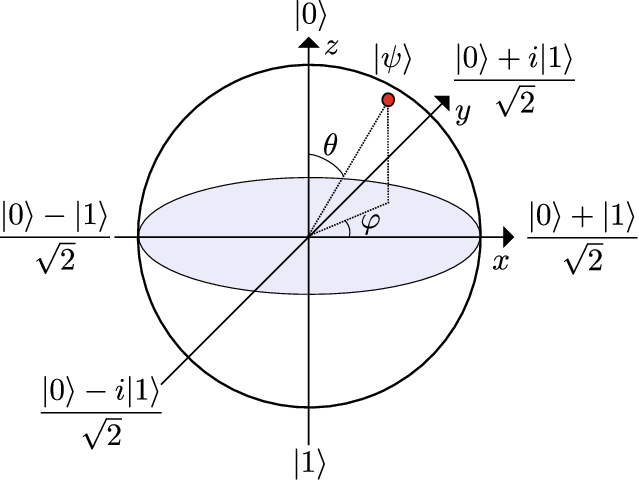
\includegraphics[width=0.9\textwidth]{gambar/BASIC/Bloch-Shapire.png}
                                \captionsetup{font=tiny} % Ukuran teks caption diset ke tiny
                                \caption{Bola Bloch}
                                \label{fig:label_gambar}
                            \end{figure}
                        \end{minipage}%
                        \begin{minipage}[c]{0.6\textwidth}
                            \tiny Bola Bloch adalah representasi geometris dari keadaan kuantum dalam mekanika kuantum yang digunakan untuk menggambarkan keadaan kuantum dari satu qubit. Setiap titik di permukaan bola Bloch mewakili satu keadaan kuantum yang mungkin dari satu qubit. Secara umum dapat dilihat melalui persamaan
                                \begin{equation}
                                    \ket{\psi} = \cos\left(\frac{\theta}{2}\right)\ket{0} + e^{i\phi}\sin\left(\frac{\theta}{2}\right)\ket{1},
                                \end{equation}   
                        \end{minipage}
                   % \end{columns}
            \end{itemize}        
        \end{column}
        
        \begin{column}{0.5\textwidth}
            \tiny di mana \(\ket{\psi}\) adalah keadaan kuantum yang diwakili oleh titik di permukaan \textit{bola Bloch}, \(\theta\) adalah sudut polar, dan \(\phi\) adalah sudut azimut.
        \end{column}
    \end{columns}
\end{frame}

%------------------------------------------------
\begin{frame}
\frametitle{Catatan 1}
    \begin{columns} %Frame Kiri
        \begin{column}{0.5\textwidth}
        \justifying % Perataan kanan kiri
        \tiny % Ukuran teks menjadi kecil
        \vspace{-0.5 cm}
            \begin{itemize}
            \justifying % Perataan kanan kiri
            \tiny % Ukuran teks menjadi kecil
                \item \textbf{Argumen Einstein-Podolsky-Rosen (EPR):}
                    \begin{itemize}      \justifying \tiny 
                        \item Pada tahun 1935 dan 1936, Schrödinger mengembangkan dan memperluas argumen Einstein-Podolsky-Rosen (EPR).
                        \item EPR merupakan kritik terhadap interpretasi mekanika kuantum Kopenhagen dan ditujukan untuk menunjukkan ketidaklengkapan teori tersebut.
                    \end{itemize}
                
                \item \textbf{Interpretasi Kopenhagen vs. Deskripsi Sistem Kuantum:}
                    \begin{itemize} \justifying \tiny 
                        \item Interpretasi Kopenhagen meyakini bahwa deskripsi suatu sistem kuantum tidak dapat dianggap sebagai daftar sifat-sifat sistem tersebut, seperti dalam mekanika klasik.
                        \item Einstein menolak pandangan ini, mengklaim bahwa keadaan kuantum suatu sistem hanya merupakan karakterisasi yang tidak lengkap.
                    \end{itemize}
                
                \item \textbf{Parameter Tersembunyi:}
                    \begin{itemize} \justifying \tiny 
                        \item Einstein menyajikan gagasan parameter tersembunyi atau variabel tersembunyi yang tidak termasuk dalam deskripsi keadaan kuantum, menunjukkan bahwa mekanika kuantum tidak memberikan gambaran lengkap.
                    \end{itemize}
                
                \item \textbf{Keterpisahan dan Lokalitas:}
                    \begin{itemize} \justifying \tiny 
                        \item Einstein tidak memandang teori yang lengkap harus bersifat deterministik, tetapi ia menetapkan kondisi keterpisahan dan lokalitas untuk sistem komposit yang terdiri dari sistem-sistem terpisah.
                    \end{itemize}
            \end{itemize} 
        \end{column}
        
            \begin{column}{0.5\textwidth} % Frame Kanan
            \justifying % Perataan kanan kiri
            \tiny % Ukuran teks menjadi kecil
            \vspace{-0.5 cm}
                \begin{itemize}
                \item \textbf{Keterjeratan Kuantum:}
                    \begin{itemize} \justifying \tiny 
                        \item Schrödinger mengusulkan konsep "keterjeratan" untuk menggambarkan hubungan aneh antara sistem kuantum yang pernah saling mempengaruhi dan kemudian terpisah.
                        \item Keterjeratan menyiratkan bahwa setelah interaksi, keadaan kedua sistem tidak dapat dijelaskan secara terpisah lagi.
                    \end{itemize}
                
                \item \textbf{Korelasi EPR:}
                    \begin{itemize} \justifying \tiny 
                        \item EPR mempertimbangkan dua partikel dalam keadaan kuantum tertentu dengan korelasi "pencocokan" antara posisi dan momentumnya.
                        \item Pengukuran pada satu partikel dapat memprediksi hasil pengukuran pada partikel lainnya.
                    \end{itemize}
                
                \item \textbf{Keterjeratan dalam Jarak Jauh:}
                    \begin{itemize} \justifying \tiny 
                        \item John Bell, pada tahun 1964, melanjutkan penelitian EPR dan menunjukkan bahwa keterjeratan dapat bertahan dalam jarak yang jauh, melemahkan ide peluruhan spontan keterjeratan.
                    \end{itemize}
                
                \item \textbf{Ketimpangan Bell:}
                    \begin{itemize} \justifying \tiny 
                        \item Ketimpangan Bell adalah inkonsistensi antara hasil pengukuran kuantum dan asumsi keterpisahan dan lokalitas Einstein.
                        \item Ini memicu perdebatan tentang dasar-dasar mekanika kuantum dan konfirmasi bahwa keterjeratan dapat terjadi pada jarak yang jauh.
                    \end{itemize}
                \end{itemize}
            \end{column}
    \end{columns}
\end{frame}

\begin{frame}
\frametitle{Catatan 2}

    \begin{columns} %Frame Kiri
        \begin{column}{0.5\textwidth}
        \justifying % Perataan kanan kiri
        \tiny % Ukuran teks menjadi kecil
            \begin{itemize}
                \item \textbf{Pandangan Baru terhadap Keterjeratan:}
                    \begin{itemize} \justifying \tiny \justifying \tiny 
                        \item Pada 1980-an, keterjeratan dianggap sebagai sumber daya fisik non-klasik yang dapat dieksploitasi, membuka jalan untuk bidang informasi kuantum.
                \end{itemize}
                \item \textbf{Pengakuan Nobel Fisika 2022:}
                    \begin{itemize} \justifying \tiny 
                        \item Alain Aspect, John F. Clauser, dan Anton Zeilinger dianugerahi Nobel Fisika 2022 atas eksperimen pada foton terjerat yang memvalidasi wawasan Bell dan memulai bidang informasi kuantum.
                \end{itemize}            
            \end{itemize} 
           Sumber catatan \firstcite{sep-qt-entangle}
        \end{column}
        
        \begin{column}{0.5\textwidth} % Frame Kanan
        %     \justifying % Perataan kanan kiri
        %     \tiny % Ukuran teks menjadi kecil
        %         \begin{itemize}
        %             \item 
        %         \end{itemize}
        \end{column}
    \end{columns}
\end{frame}

\begin{frame}
\frametitle{QUANTUM ENTANGLEMENT \cite{muller2023}}
    \begin{columns} %Frame Kiri
                \justifying % Perataan kanan kiri
            \tiny % Ukuran teks menjadi kecil
        \begin{column}{0.5\textwidth} \vspace{-0.4cm}
        \justifying % Perataan kanan kiri
        \small % Ukuran teks menjadi kecil
            \begin{itemize}\justifying \tiny
                \item EPR\\
                    Pada tahun 1935, Albert Einstein, Boris Podolsky, dan Nathan Rosen menerbitkan sebuah makalah yang menggambarkan sebuah eksperimen pemikiran yang dirancang untuk mengilustrasikan ketidak masukakalan dari quantum entanglement yang menantang hukum dasar alam semesta.
                \item Quantum Entanglement\\
                    Secara sederhana quantum entanglement merupakan rujukan pada aspek-aspek satu partikel dari sepasang partikel yang terjerat yang memiliki ketergantungan pada aspek-aspek dari partikel lainnya, dengan tidak memperdulikan seberapa jauh jaraknya atau apa yang ada di antara keduanya. 
                \item Bentuk Partikel\\
                    Partikel-partikel yang terjerat dapat berupa, elektron atau foton dan aspeknya dapat berupa keadaan partikel tersebut, seperti apakah partikel tersebut berputar ke satu arah atau ke arah lain.
                \item Pengukuran\\
                    Apabila suatu partiket terikat (ter-entanglement) maka kita dapat mengetahui ukuran partikel dengan cara mengukur salah satu pasangan yang telah terikat dan informasi tentang pasangan lainnya dapat segera diketahui, bahkan kedua pasangan partikel tersebut terpisah jutaan tahun cahaya.
            \end{itemize} 
        \end{column}
        
        \begin{column}{0.5\textwidth} \vspace{-0.3cm}% Frame Kanan
            \justifying % Perataan kanan kiri
            \tiny % Ukuran teks menjadi kecil
                \begin{itemize}
                \item Superposisi\\
                    Superposisi kuantum merupakan suatu gagasan tentang partikel yang berada dalam beberapa keadaan sekaligus, akan tetapi ketika dilakukan pengukuran partiker akan memilih salah satu keadaan dalam superposisi.
                \item Cara Pertikel Terjerat\\
                    Secara sederhana dasar membuat partikel terjerat dilakukan dengan cara memecah sistem menjadi dua dnegan jumlah bagian-bagiannya diketahui. Contoh, kita bisa membagi sebuah partikel dengan spin nol menjadi dua partikel yang memiliki spin berlawanan sehingga jumlah keduanya adalah nol. 
                \item Runtuhnya Probabilitas\\
                    Dalam mekanika kuantum, spin setiap partikel adalah sebagian naik dan sebagian turun sampai diukur. Hanya ketika pengukuran terjadi, keadaan kuantum spin “runtuh” menjadi naik atau turun seketika meruntuhkan partikel lainnya ke spin yang berlawanan. 
                \item Variabel Tersembunyi\\
                    Einstein berteori bahwa ada beberapa properti yang tidak diketahui dijuluki sebagai variabel tersembunyi yang menentukan keadaan partikel sebelum pengukuran.
                \item  Persamaan Bell\\
                    Bell menghasilkan sebuah persamaan yang sekarang dikenal sebagai bell's inequality yang selalu benar dan yang hanya benar untuk teori-teori variabel tersembunyi, dan tidak selalu benar untuk mekanika kuantum.  
                \end{itemize}
        \end{column}
    \end{columns}
\end{frame}